\section{Objects in the amber.showoff package}


\classname{EarthView}

\begin{classmetadata}
  \extends{javax.swing.JPanel}
  \implements{Runnable}
  \dependencies{FullScreen, StoryLauncher}
  \function{EarthView is a graphical user interface element based on a JPanel
      which displays a picture of Earth in space, with particles orbiting
      around it. Attractors can be added to influence the orbits of the
      particles.}
  \processing{There is a list of particles, which contains information on
      their location and more. EarthView draws each of the particles in the
      list on itself.}
\end{classmetadata}

\begin{interface}
  \init{EarthView}{Collection$\langle$Particle$\rangle$ pc}
    {Initializes the EarthView display. It is a child of JPanel and can as such
    be used inside any Swing application. Before starting the Earthview, first
    couple a Particle collection to it using setParticleCollection.}
  \method{\void}{setParticleCollection}{pc: Collection$\langle$Particle$\rangle$}
    {Sets the collection of particles to be displayed in the view.}
  \method{\void}{run}{}
    {Runs the thread (for Runnable).}
  \method{\void}{start}{}
    {Starts the thread, lets EarthView draw stuff.}
\end{interface}



\classname{FullScreen}

\begin{classmetadata}
  \extends{amber.ShowOffObject}
  \implements{amber.common.AirBrushCallable}
  \dependencies{ShowOff}
  \function{This is a ShowOff module which displays the visualization in full
    screen size.}
\end{classmetadata}

\begin{interface}
  \init{FullScreen}{}
    {Initializes something.}
  \method{\void}{start}{}
    {Start the visualization.}
\end{interface}



\classname{Particle}

\begin{classmetadata}
  \function{Storage of particle data.}
  \data{An object of this class has information about its location and
    velocity, and it knows from which story it originates.}
  \dependencies{StoryLauncher, Particles}
\end{classmetadata}

\begin{interface}
  \init{Particle}{Story s}
    {Initializes a particle for Story s.}
  \method{\void}{launch}{}
    {Launches the particle, all parameters must be set, they cannot be changed
      afterwards.}
  \method{\void}{boost}{double}
    {Boost the particle in the direction it is heading. This can happen when
      for instance the Story gets replies or comments; boosting keeps the
      particle around longer.}
  \method{double}{getMass}{}
    {Gets the mass of the particle}
  \method{Point2d}{getLocation}{}
    {Gets the location}
  \method{Vector2d}{getVelocity}{}
    {Gets the velocity}
  \method{Vector2d}{getAcceleration}{}
    {Gets the acceleration}
  \method{\void}{setMass}{double s}
    {Sets the mass of the particle to s}
  \method{\void}{setLocation}{Point2d v}
    {Sets the location to v}
  \method{\void}{setVelocity}{Vector2d v}
    {Sets the velocity to v}
  \method{\void}{setAcceleration}{Vector2d v}
    {Sets the acceleration to v}
  \method{\void}{setNewValuesAfter}{double t}
    {Calculates and sets new values using the current values after a period of
      time t}
\end{interface}



\classname{Applet}

\begin{classmetadata}
  \extends{java.applet.Applet}
\end{classmetadata}

\begin{interface}
\end{interface}



\begin{figure}
  \centering
  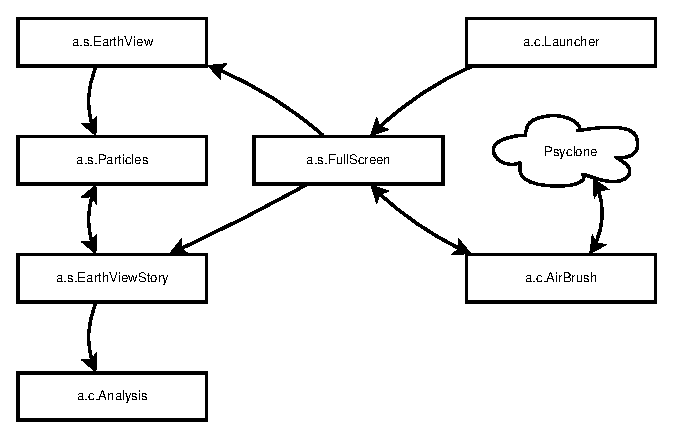
\includegraphics{image/showoff-fullscreen}
  \caption{
    Diagram of the design of the full screen ShowOff module, the names are
    abbreviated Java classnames
  }
\end{figure}

